% March 2015
% Autor: Mandy Vogel
% introduction

\documentclass[xcolor={table},c]{beamer}
%\usetheme[backgroundimagefile=mathe]{diepen}
\usetheme{Singapore}
% \useoutertheme{miniframes}

%\setbeamerfont{block title}{size=\small,series=\bfseries}
%\setbeamerfont{block body}{size=\footnotesize}

% \usecolortheme{beetle}
\usepackage{linkimage}

%\usepackage{handoutWithNotes}
%\pgfpagesuselayout{3 on 1 with notes}[a4paper,border shrink=5mm]

\begin{document}

\title{Introduction}   
\author{Mandy Vogel} 
\date{\today}

\AtBeginSection{
  \begin{frame}<beamer>[allowframebreaks,t]{Table of Contents}
    \tableofcontents[currentsection]
  \end{frame}}

\begin{frame}
\titlepage
\end{frame}

\begin{frame}[allowframebreaks,t]{Table of Contents}
\frametitle{Table of Contents}\tableofcontents
\end{frame}

\section{Remember!}
\subsection{Implicit Loops}
\begin{frame}[fragile]\frametitle{Implicit Loops}
A common application of loops is  to apply a function to each element of a set of values and collect the results in a single structure.

In R this is done by the functions:
\begin{itemize}
 \item \texttt{lapply()} - works on elements of a list
 \item \texttt{sapply()} - same as lapply but simplify results
 \item \texttt{apply()} - works on rows or colums of a matrix or a data frame (or more general on arrays)
 \item \texttt{tapply()} - works on groups defined by an index
\end{itemize}
\end{frame}


\subsection{Exercises}
\begin{frame}[fragile,allowframebreaks]\frametitle{\texttt{\texttt{apply()} Exercises}}
Given the two R object \texttt{m} and \texttt{l} below use
  \begin{enumerate}
  \item  use \texttt{lapply()} to get the class and the length of each element of \texttt{l} (two steps)
  \item  \texttt{apply()} to get the maximum of each column in \texttt{m}
\begin{verbatim}
> m <- matrix(1:100, nrow=10)
> l <- list(a=1:10,b=rep(c(T,F),2),c=letters)  
\end{verbatim}
  \end{enumerate}
\end{frame}


\section{\texttt{read.file()} again}
\subsection{\texttt{read.file()}}
\begin{frame}[fragile]\frametitle{\texttt{read one file}}
\begin{verbatim}
> file <- "../session1/session1data/pre001.txt"
> pre1 <- read.file(file,skip=3)
[1] "read ../session1/session1data/pre001.txt"
> file <- "data/pretest/pre_001.txt"
> pre1v2 <- read.file(file,skip=0)
[1] "read ../session2/data/pretest/pre_001.txt"
\end{verbatim}
\end{frame}


\begin{frame}[fragile]\frametitle{\texttt{read several files}}
  \begin{itemize}
  \item we used \texttt{dir()} (with the arguments \texttt{pattern}, \texttt{recursive}, \texttt{full.path}) to get a list of file names we wanted to read in 
  \item we learned about \texttt{lapply()} which takes a list l and a function f to perform the function f on every element of the list l
  \item so now we combine what we learned to read all files at once
  \end{itemize}
\end{frame}


\begin{frame}[fragile]\frametitle{\texttt{read several files}}
\begin{verbatim}
  > files <- dir("../session2/data",full.names = T, 
+                recursive = T,pattern = "txt$")
  > files
  [1] "../session2/data/posttest/post_001.txt"   
  [2] "../session2/data/posttest/post_002.txt"   
  [3] "../session2/data/posttest/post_003.txt"   
  [4] "../session2/data/posttest/post_004.txt"   
  [5] "../session2/data/posttest/post_005.txt"   
  [6] "../session2/data/posttest/post_006.txt"   
  [7] "../session2/data/posttest/post_007.txt"   
...
\end{verbatim}
\end{frame}


\begin{frame}[fragile]\frametitle{\texttt{get files names}}
\begin{verbatim}
  > files <- dir("../session2/data",full.names = T, 
+                recursive = T,pattern = "txt$")
  > files
  [1] "../session2/data/posttest/post_001.txt"   
  [2] "../session2/data/posttest/post_002.txt"   
  [3] "../session2/data/posttest/post_003.txt"   
  [4] "../session2/data/posttest/post_004.txt"   
  [5] "../session2/data/posttest/post_005.txt"   
  [6] "../session2/data/posttest/post_006.txt"   
  [7] "../session2/data/posttest/post_007.txt"   
...
\end{verbatim}
\end{frame}

\begin{frame}[fragile]\frametitle{\texttt{read in files}}
  \begin{itemize}
  \item source the file containing our function \texttt{read.file()}
  \item use \texttt{lapply()} to use \texttt{read.file()} on every entry of the list of file names
  \end{itemize}
\begin{verbatim}
  > source("function.r")
  > df.list <- lapply(files,read.file,skip=0)
  [1] "read ../session2/data/posttest/post_001.txt"
  [1] "read ../session2/data/posttest/post_002.txt"
  [1] "read ../session2/data/posttest/post_003.txt"
  [1] "read ../session2/data/posttest/post_004.txt"
  [1] "read ../session2/data/posttest/post_005.txt"
  [1] "read ../session2/data/posttest/post_006.txt"
  [1] "read ../session2/data/posttest/post_007.txt"
  [1] "read ../session2/data/posttest/post_008.txt"
...
\end{verbatim}
\end{frame}


\begin{frame}[fragile]\frametitle{Result}
\begin{itemize}
\item what we get is a list \texttt{df.list} containing the results: every element of the list is a data frame if \texttt{read.file()} read in successfully the respective file
\item so our variable \texttt{files} contains 195 file names
\begin{verbatim}
> length(files)
[1] 195  
\end{verbatim}
\item so \texttt{df.list} contains 195 elements
\begin{verbatim}
> length(df.list)
[1] 195  
\end{verbatim}
\item we can check the class of each of these results again with \texttt{sapply()}
\begin{verbatim}
> table(sapply(df.list,class))

data.frame       NULL 
       192          3   
\end{verbatim}
\end{itemize}
\end{frame}


\subsection{Remember!}
\begin{frame}[fragile]\frametitle{\texttt{Combining Data Frames}}
We learned about three basis functions to combine data frame
\begin{itemize}
\item \texttt{rbind()} - combine two data frames row wise
\item \texttt{cbind()} - combine two data frames column wise
\item \texttt{merge()} - combine two data with respect two one or more identifying columns
\end{itemize}
\end{frame}


\begin{frame}[fragile]\frametitle{\texttt{Combining Data Frames}}
\begin{itemize}
\item all of them are binary function
\item so you can not put more than two data frame into it
\item using only these function it would be a tedious and boring work to combine 192 data frames
\end{itemize}
\end{frame}


\subsection{\texttt{Reduce()}}
\begin{frame}[fragile]\frametitle{\texttt{Reduce()}}
\begin{itemize}
\item is also a higher order function (functional)
\item \texttt{Reduce()} uses a binary function (like \texttt{rbind()} or \texttt{merge()}) to combine successively the elements of a given list
\item it can be used if you have not only two but many data frames
\end{itemize}
\end{frame}


\begin{frame}[fragile]\frametitle{\texttt{Reduce()}}
  \begin{itemize}
  \item first we make up 4 artifical data frames
  \end{itemize}
\end{frame}


\begin{frame}[fragile]\frametitle{\texttt{Reduce()}}
\begin{verbatim}\tiny
> (d1 <- data.frame(id=LETTERS[c(1,2,3)],day1=sample(10,3)))
  id day1
1  A    3
2  B    1
3  C    7
> (d2 <- data.frame(id=LETTERS[c(1,3,5,6)],day2=sample(10,4)))
  id day2
1  A    8
2  C    2
3  E    5
4  F    3
> (d3 <- data.frame(id=LETTERS[c(2,4:6)],day3=sample(10,4)))
  id day3
1  B    8
2  D    3
3  E    4
4  F   10
> (d4 <- data.frame(id=LETTERS[c(1:5)],day4=sample(10,5)))
  id day4
1  A    2
2  B    7
3  C    8
4  D    9
5  E    1
\end{verbatim}
\end{frame}

\begin{frame}[fragile]\frametitle{\texttt{Reduce()}}
  \begin{itemize}
  \item now we use \texttt{Reduce()} in combination with \texttt{merge()}
  \begin{exampleblock}{Input/Output}\tiny
\begin{verbatim}
> Reduce(merge,list(d1,d2,d3,d4))
[1] id   day1 day2 day3 day4
<0 Zeilen> (oder row.names mit Länge 0)
\end{verbatim}
  \end{exampleblock}
\item and what we get is an empty data frame
\item well this isn't exactly what we wanted, so why?
\item it is because the default behavior of \texttt{merge()} is set \texttt{all=F}, so we get only complete lines which is in this case - none
\item so we have to define a wrapper function which only change this argument to \texttt{all=T}
  \end{itemize}

\end{frame}


\begin{frame}[fragile]\frametitle{\texttt{Reduce()}}
  \begin{itemize}
  \item now we use \texttt{Reduce()} in combination with \texttt{merge()}
  \begin{exampleblock}{Input/Output}\small
\begin{verbatim}
> Reduce(function(x,y) { merge(x,y, all=T) },
+        list(d1,d2,d3,d4))
  id day1 day2 day3 day4
1  A    3    8   NA    2
2  B    1   NA    8    7
3  C    7    2   NA    8
4  E   NA    5    4    1
5  F   NA    3   10   NA
6  D   NA   NA    3    9
\end{verbatim}
  \end{exampleblock}
\item which is exactly what we want
  \end{itemize}
\end{frame}

\begin{frame}[fragile]\frametitle{\texttt{Reduce()}}
  \begin{itemize}
  \item a second example in combination with \texttt{rbind()}
  \begin{exampleblock}{Input/Output}\small
\begin{verbatim}
> d4$day <- names(d4)[2]
> names(d4)[2] <- "score"
> Reduce(function(x,y) { y$day <- names(y)[2]
+                        names(y)[2] <- "score"
+                        rbind(x,y) } ,
+        list(d1,d2,d3), init = d4)
   id score  day
1   A     2 day4
2   B     7 day4
3   C     8 day4
4   D     9 day4
...
\end{verbatim}
  \end{exampleblock}
\item which is exactly what we want
  \end{itemize}
\end{frame}


\begin{frame}[fragile]\frametitle{\texttt{Reduce() Exercise}}
  \begin{itemize}
  \item the list \texttt{ml} contains three vectors
  \item use \texttt{lapply()} to get the class of each of them
  \item then use \texttt{Reduce()} and combination with \texttt{c()} to coerce them into one vector. Of which class is the resulting vector?
  \end{itemize}
\begin{verbatim}
> ml <- list(vl <- c(TRUE,FALSE),
+            vn <- 1:10,
+            vc <- letters)
\end{verbatim}
\end{frame}



\begin{frame}[fragile]\frametitle{\texttt{Reduce() Exercise}}
  \begin{itemize}
  \item use \texttt{lapply()} to get the class of each of them

  \scriptsize
\begin{verbatim}
> lapply(ml,class)
[[1]]
[1] "logical"

[[2]]
[1] "integer"

[[3]]
[1] "character"
\end{verbatim} 
\normalsize
  \item then use \texttt{Reduce()} and combination with \texttt{c()} to coerce them into one vector. Of which class is the resulting vector?
\scriptsize
\begin{verbatim}
> rv <- Reduce(c,ml)
> rv
 [1] "1"  "0"  "1"  "2"  "3"  "4"  "5"  "6"  "7"  "8"  "9"  "10" "a"  "b"  "c" 
[16] "d"  "e"  "f"  "g"  "h"  "i"  "j"  "k"  "l"  "m"  "n"  "o"  "p"  "q"  "r" 
[31] "s"  "t"  "u"  "v"  "w"  "x"  "y"  "z" 
> class(rv)
[1] "character"
\end{verbatim}
\end{itemize}
\end{frame}


\begin{frame}[fragile]\frametitle{Combine all data frames}
  \begin{itemize}
  \item We used \texttt{lapply()} and our function \texttt{read.file()} to read all files in \texttt{files}
  \item and we got back a list \texttt{df.list} containing 192 data frames
\begin{verbatim}
> df.list <- lapply(files,read.file,skip=0)
[1] "read data/posttest/post_001.txt"
[1] "read data/posttest/post_002.txt"
[1] "read data/posttest/post_003.txt"
[1] "read data/posttest/post_004.txt"
[1] "read data/posttest/post_005.txt"
...
> table(sapply(df.list,class))

data.frame       NULL 
       192          3   
\end{verbatim}
  \end{itemize}
\end{frame}



\begin{frame}[fragile]\frametitle{Combine all data frames - exercise}
  \begin{itemize}
  \item now use what we learned about  \texttt{Reduce{}} and combining data frames using \texttt{rbind()}  to combine these 192 data frames. 

  \end{itemize}
\end{frame}

\begin{frame}[fragile]\frametitle{Combine all data frames - exercise}
\tiny
\begin{verbatim}
> data <- Reduce(rbind,df.list)
> nrow(data)
[1] 12704
> table(data$Subject)

001_test2 002_test2 003_test2 004_test2 005_test2 006_test2 007_test2 008_test2 
       93        91        96        93        95        95        93        96 
009_test2 010_test2 011_test2 012_test2 013_test2 014_test2 015_test2 016_test2 
       92        94        95        96        96        95        96        94 
017_test2 018_test2 019_test2 020_test2 001_test1 002_test1 003_test1 004_test1 
       95        94        96        95        95        95        96        94 
005_test1 006_test1 007_test1 008_test1 009_test1 010_test1 011_test1 012_test1 
       96        95        94        90        96        95        91        96 
013_test1 014_test1 015_test1 016_test1 017_test1 018_test1 019_test1 020_test1 
       95        96        95        91        96        96        96        96 
    001_1     002_1     003_1     004_1     005_1     006_1    CHGU_1    008_1a 
       60        59        60        54        60        59        60        60 
    009_1     010_1     RMK_1     013_1     014_1     015_1     016_1    IJ2K_1 
       60        60        59        59        60        58        59        58 
    018_1     019_1     020_1     001_2     002_2     003_2     004_2     005_2 
       60        59        60        59        59        57        58        57 
    006_2     007_2     008_2     009_2     010_2     011_2     012_2     013_2 
       58        58        54        58        58        59        59        56 
    014_2     015_2     016_2     017_2     018_2     019_2     020_2     001_3 
...
\end{verbatim}
\end{frame}


\begin{frame}[fragile]\frametitle{The Function no 2}
  \begin{itemize}
  \item so it is recommended to build again a function out of this
    \begin{exampleblock}{Input/Output}\scriptsize
\begin{verbatim}
> read.files <- function(filesdir,skip=3,recursive=F,pattern="."){
+     files <- dir(filesdir,
+                  full.names = T,
+                  recursive = recursive,
+                  pattern = pattern)
+     Reduce(rbind,lapply(files,read.file,skip=skip))}
> data <- read.files("data",recursive = T,skip=0,pattern = "\\.txt$")
[1] "read data/posttest/post_001.txt"
[1] "read data/posttest/post_002.txt"
[1] "read data/posttest/post_003.txt"
[1] "read data/posttest/post_004.txt"
[1] "read data/posttest/post_005.txt"
...
\end{verbatim}
    \end{exampleblock}
  \end{itemize}
\end{frame}



\begin{frame}[fragile]\frametitle{The Function no 2}
  \begin{itemize}
  \item by changing the pattern (passed through to \texttt{dir()} we can limit the read in files to specific time or person\tiny
\begin{verbatim}
## only person 002
> sub1 <- read.files("../session2/data",
+                    skip = 0, recursive = T,pattern="\\002\\.txt$")
[1] "read ../session2/data/posttest/post_002.txt"
[1] "read ../session2/data/pretest/pre_002.txt"
[1] "read ../session2/data/training_1/train_002.txt"
[1] "read ../session2/data/training_2/train_002.txt"
[1] "read ../session2/data/training_3/train_002.txt"
...
## only test
> test <- read.files("../session2/data",
+                    skip = 0, recursive = T,pattern="p[ro].+\\.txt$")
[1] "read ../session2/data/posttest/post_001.txt"
[1] "read ../session2/data/posttest/post_002.txt"
...
[1] "read ../session2/data/pretest/pre_001.txt"
[1] "read ../session2/data/pretest/pre_002.txt"
...
\end{verbatim}
  \end{itemize}
\end{frame}


\section{Exploratory Analysis}
\subsection{Variable Coding}
\begin{frame}[fragile]\frametitle{The \texttt{Subject} column}
  \begin{itemize}
  \item table the \texttt{Subject} column again. What is the problem?
  \end{itemize}
\end{frame}


\begin{frame}[fragile]\frametitle{The \texttt{Subject} column}
\begin{exampleblock}{Input/Output}\scriptsize
\begin{verbatim}
> table(data$Subject)

001_test2 002_test2 003_test2 004_test2 005_test2 006_test2 007_test2 008_test2 
       93        91        96        93        95        95        93        96 
009_test2 010_test2 011_test2 012_test2 013_test2 014_test2 015_test2 016_test2 
       92        94        95        96        96        95        96        94 
017_test2 018_test2 019_test2 020_test2 001_test1 002_test1 003_test1 004_test1 
       95        94        96        95        95        95        96        94 
...
\end{verbatim}
    \end{exampleblock}
\begin{itemize}
\item subject and time coded in one variable
\end{itemize}
\end{frame}



\begin{frame}[fragile]\frametitle{The \texttt{Subject} column}
  \begin{itemize}
  \item we create two new variables using the \texttt{str\_split()} function (stringr package)
  \item because \texttt{str\_split()} has a list containing a vector as result we have to use it in combination with \texttt{sapply()}
  \item then correct some of the person ids
  \end{itemize}
\begin{exampleblock}{Input/Output}\small
\begin{verbatim}
> data$persid <- sapply(data$Subject,function(x)
+     str_split(x,pattern = "_")[[1]][1])
> data$testid <- sapply(data$Subject,function(x)
+     str_split(x,pattern = "_")[[1]][2])
\end{verbatim}
    \end{exampleblock}
\end{frame}


\begin{frame}[fragile]\frametitle{The \texttt{Subject} column}
  \begin{itemize}
  \item a alternative is using again regular expressions using the \texttt{str\_replace()} function (again stringr package)
  \item \texttt{str\_replace()} takes three arguments: the string, the pattern to be replaced and the replacement
  \end{itemize}
\begin{exampleblock}{Input/Output}\small
\begin{verbatim}
> data$testid <- str_replace(data$Subject,"^.+_","")
> data$persid <- str_replace(data$Subject,"_.+$","")
> data$Subject <- NULL
> data$persid[data$persid=="CHGU"] <- "007"
\end{verbatim}
    \end{exampleblock}
\end{frame}



\begin{frame}[fragile]\frametitle{The \texttt{Subject} column Exercises}
  \begin{itemize}
  \item there are some more wrong person ids: RMK - 011, IJ2K - 017, GA3K - 004, Kj6K - 006. Correct them!
  \end{itemize}
\end{frame}

\begin{frame}[fragile]\frametitle{The \texttt{Subject} column Exercises}
\begin{exampleblock}{Input/Output}\small
\begin{verbatim}
> data$persid[data$persid=="RMK"] <- "011"
> data$persid[data$persid=="IJ2K"] <- "017"
> data$persid[data$persid=="GA3K"] <- "004"
> data$persid[data$persid=="Kj6K"] <- "006"
\end{verbatim}
    \end{exampleblock}
\end{frame}


\begin{frame}[fragile]\frametitle{Merging}
  \begin{enumerate}
  \item now read in the file subjectsdemographics.txt using the appropriate command
  \item join the demographics with our data data frame (there is a little problem left - compare the persid and Subject columns)
  \end{enumerate}
\end{frame}


\begin{frame}[fragile]\frametitle{The \texttt{Subject} column Exercises}
\begin{verbatim}
> persdat <- read.table("data/subjectdemographics.txt",
+                       sep="\t",
+                       header=T)
> persdat$Subject
 [1]  1  2  3  4  5  6  7  8  9 10 11 12 13 14 15 16 17 18 19 20
> unique(data$persid)
 [1] "001" "002" "003" "004" "005" "006" "007" "008" "009" "010" "011" "012"
[13] "013" "014" "015" "016" "017" "018" "019" "020"
> data$persid <- as.numeric(data$persid)
> unique(data$persid)
 [1]  1  2  3  4  5  6  7  8  9 10 11 12 13 14 15 16 17 18 19 20
> data <- merge(persdat,data,by.x = "Subject",by.y = "persid",all=T)
> head(data)
> summary(data)
    Subject      Sex       Age_PRETEST        Trial          Event.Type   
 Min.   : 1.00   f:7658   Min.   :3.100   Min.   :  7.0   Picture :    0  
 1st Qu.: 5.00   m:5046   1st Qu.:3.110   1st Qu.:112.0   Response:12704  
 Median :11.00            Median :4.400   Median :222.0   Sound   :    0  
 Mean   :10.53            Mean   :4.154   Mean   :223.1   Pause   :    0  
 3rd Qu.:16.00            3rd Qu.:4.600   3rd Qu.:332.0   Resume  :    0  
 Max.   :20.00            Max.   :4.900   Max.   :482.0   Video   :    0  
...
\end{verbatim}
\end{frame}


\subsection{Summary graphs}
\begin{frame}[fragile]\frametitle{Summary Graphics}
Just run the code and try to understand it. We will cover the ggplot graphics soon.
\begin{exampleblock}{Input/Output}\tiny
\begin{verbatim}
> ggplot(data,aes(x=factor(Subject),fill=..count..)) +
+     geom_bar() +
+     facet_wrap(~testid)
\end{verbatim}
    \end{exampleblock}
\begin{center}
  \linkimage{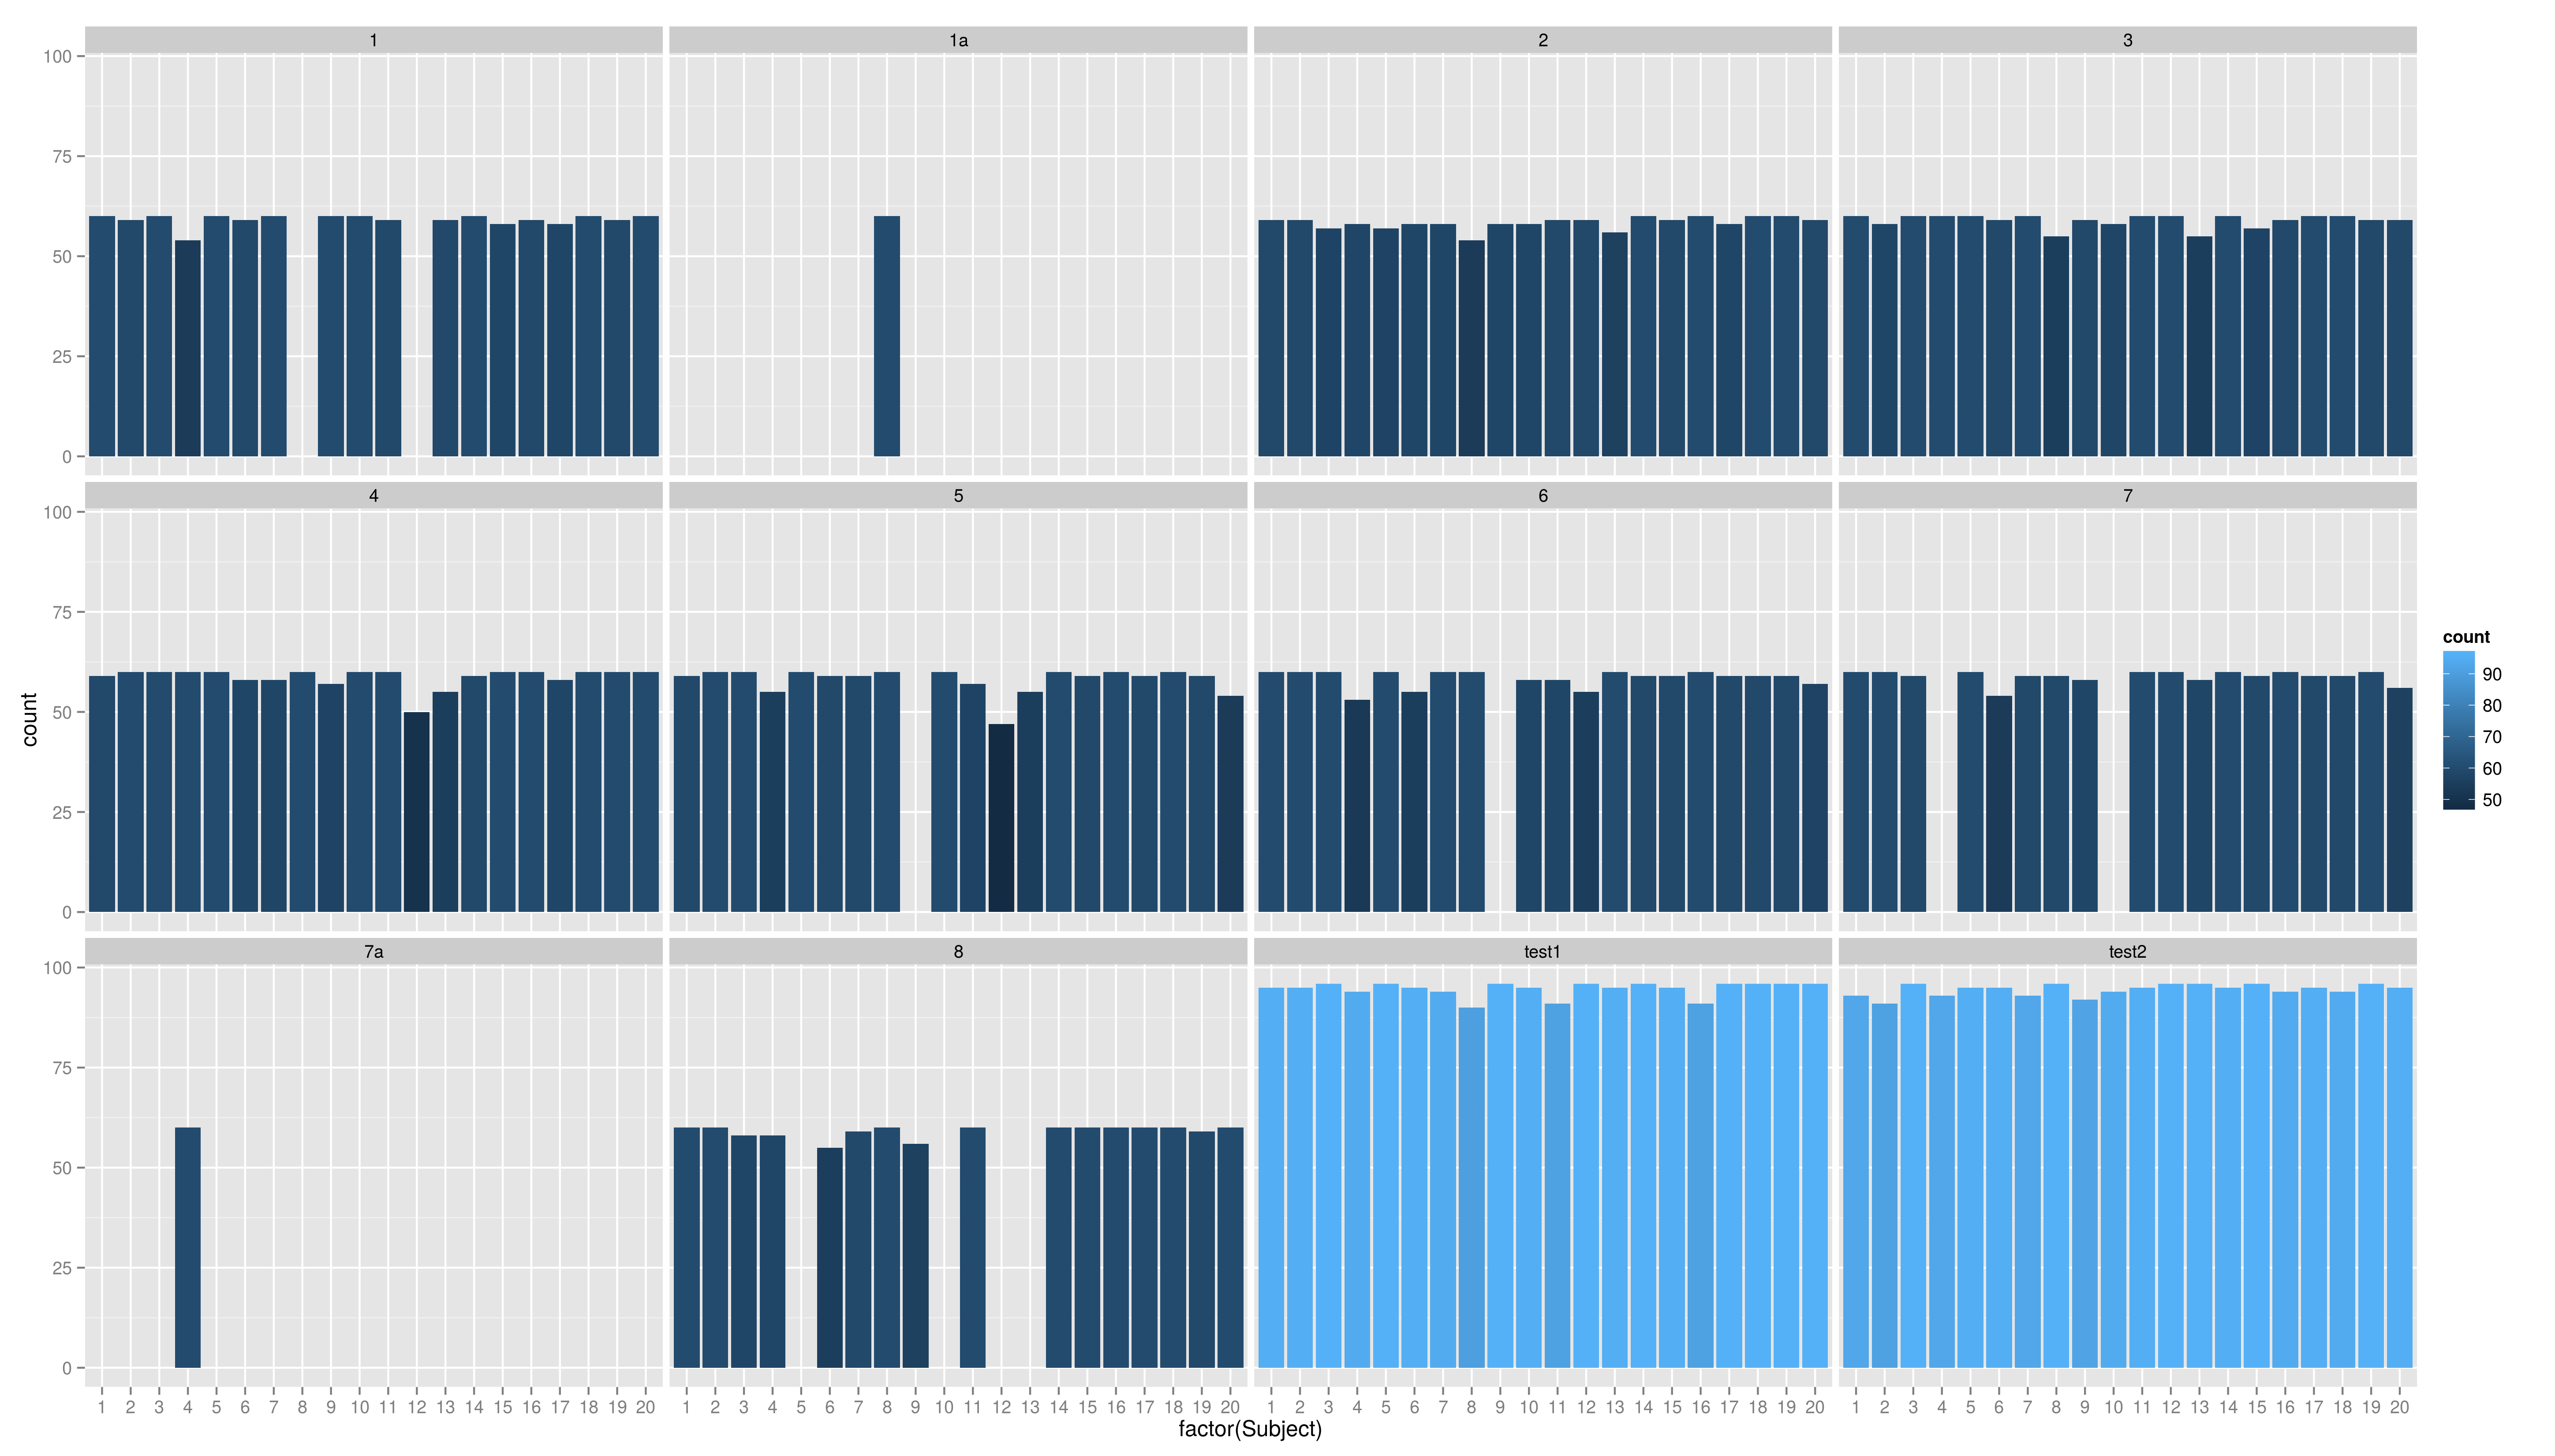
\includegraphics[width=8cm, height=4cm]{graph1.png}}{graph1.png}
\end{center}
\end{frame}

\begin{frame}[fragile]\frametitle{Summary Graphics}
  \begin{itemize}
  \item so there are problems in coding of the test id
  \item we remove the letters at the end using \texttt{str\_replace()}
  \end{itemize}\footnotesize
\begin{verbatim}
> data$testid <- str_replace(data$testid,"[a-z]$","")
> data$testid <- factor(data$testid,
+                       levels=c("test1","1","2","3","4","5","6","7","8","test2"))
> table(data$Subject,data$testid)
    
     test1  1  2  3  4  5  6  7  8 test2
  1     95 60 59 60 59 59 60 60 60    93
  2     95 59 59 58 60 60 60 60 60    91
  3     96 60 57 60 60 60 60 59 58    96
  4     94 54 58 60 60 55 53 60 58    93
  5     96 60 57 60 60 60 60 60  0    95
  6     95 59 58 59 58 59 55 54 55    95
  7     94 60 58 60 58 59 60 59 59    93
  8     90 60 54 55 60 60 60 59 60    96
  9     96 60 58 59 57  0  0 58 56    92
...
\end{verbatim}
\end{frame}


\begin{frame}[fragile]\frametitle{Summary Graphics}
\begin{exampleblock}{Input/Output}\tiny
\begin{verbatim}
> ggplot(data,aes(x=factor(Subject),fill=..count..)) +
+     geom_bar() +
+     facet_wrap(~testid)
\end{verbatim}
    \end{exampleblock}
\begin{center}
  \linkimage{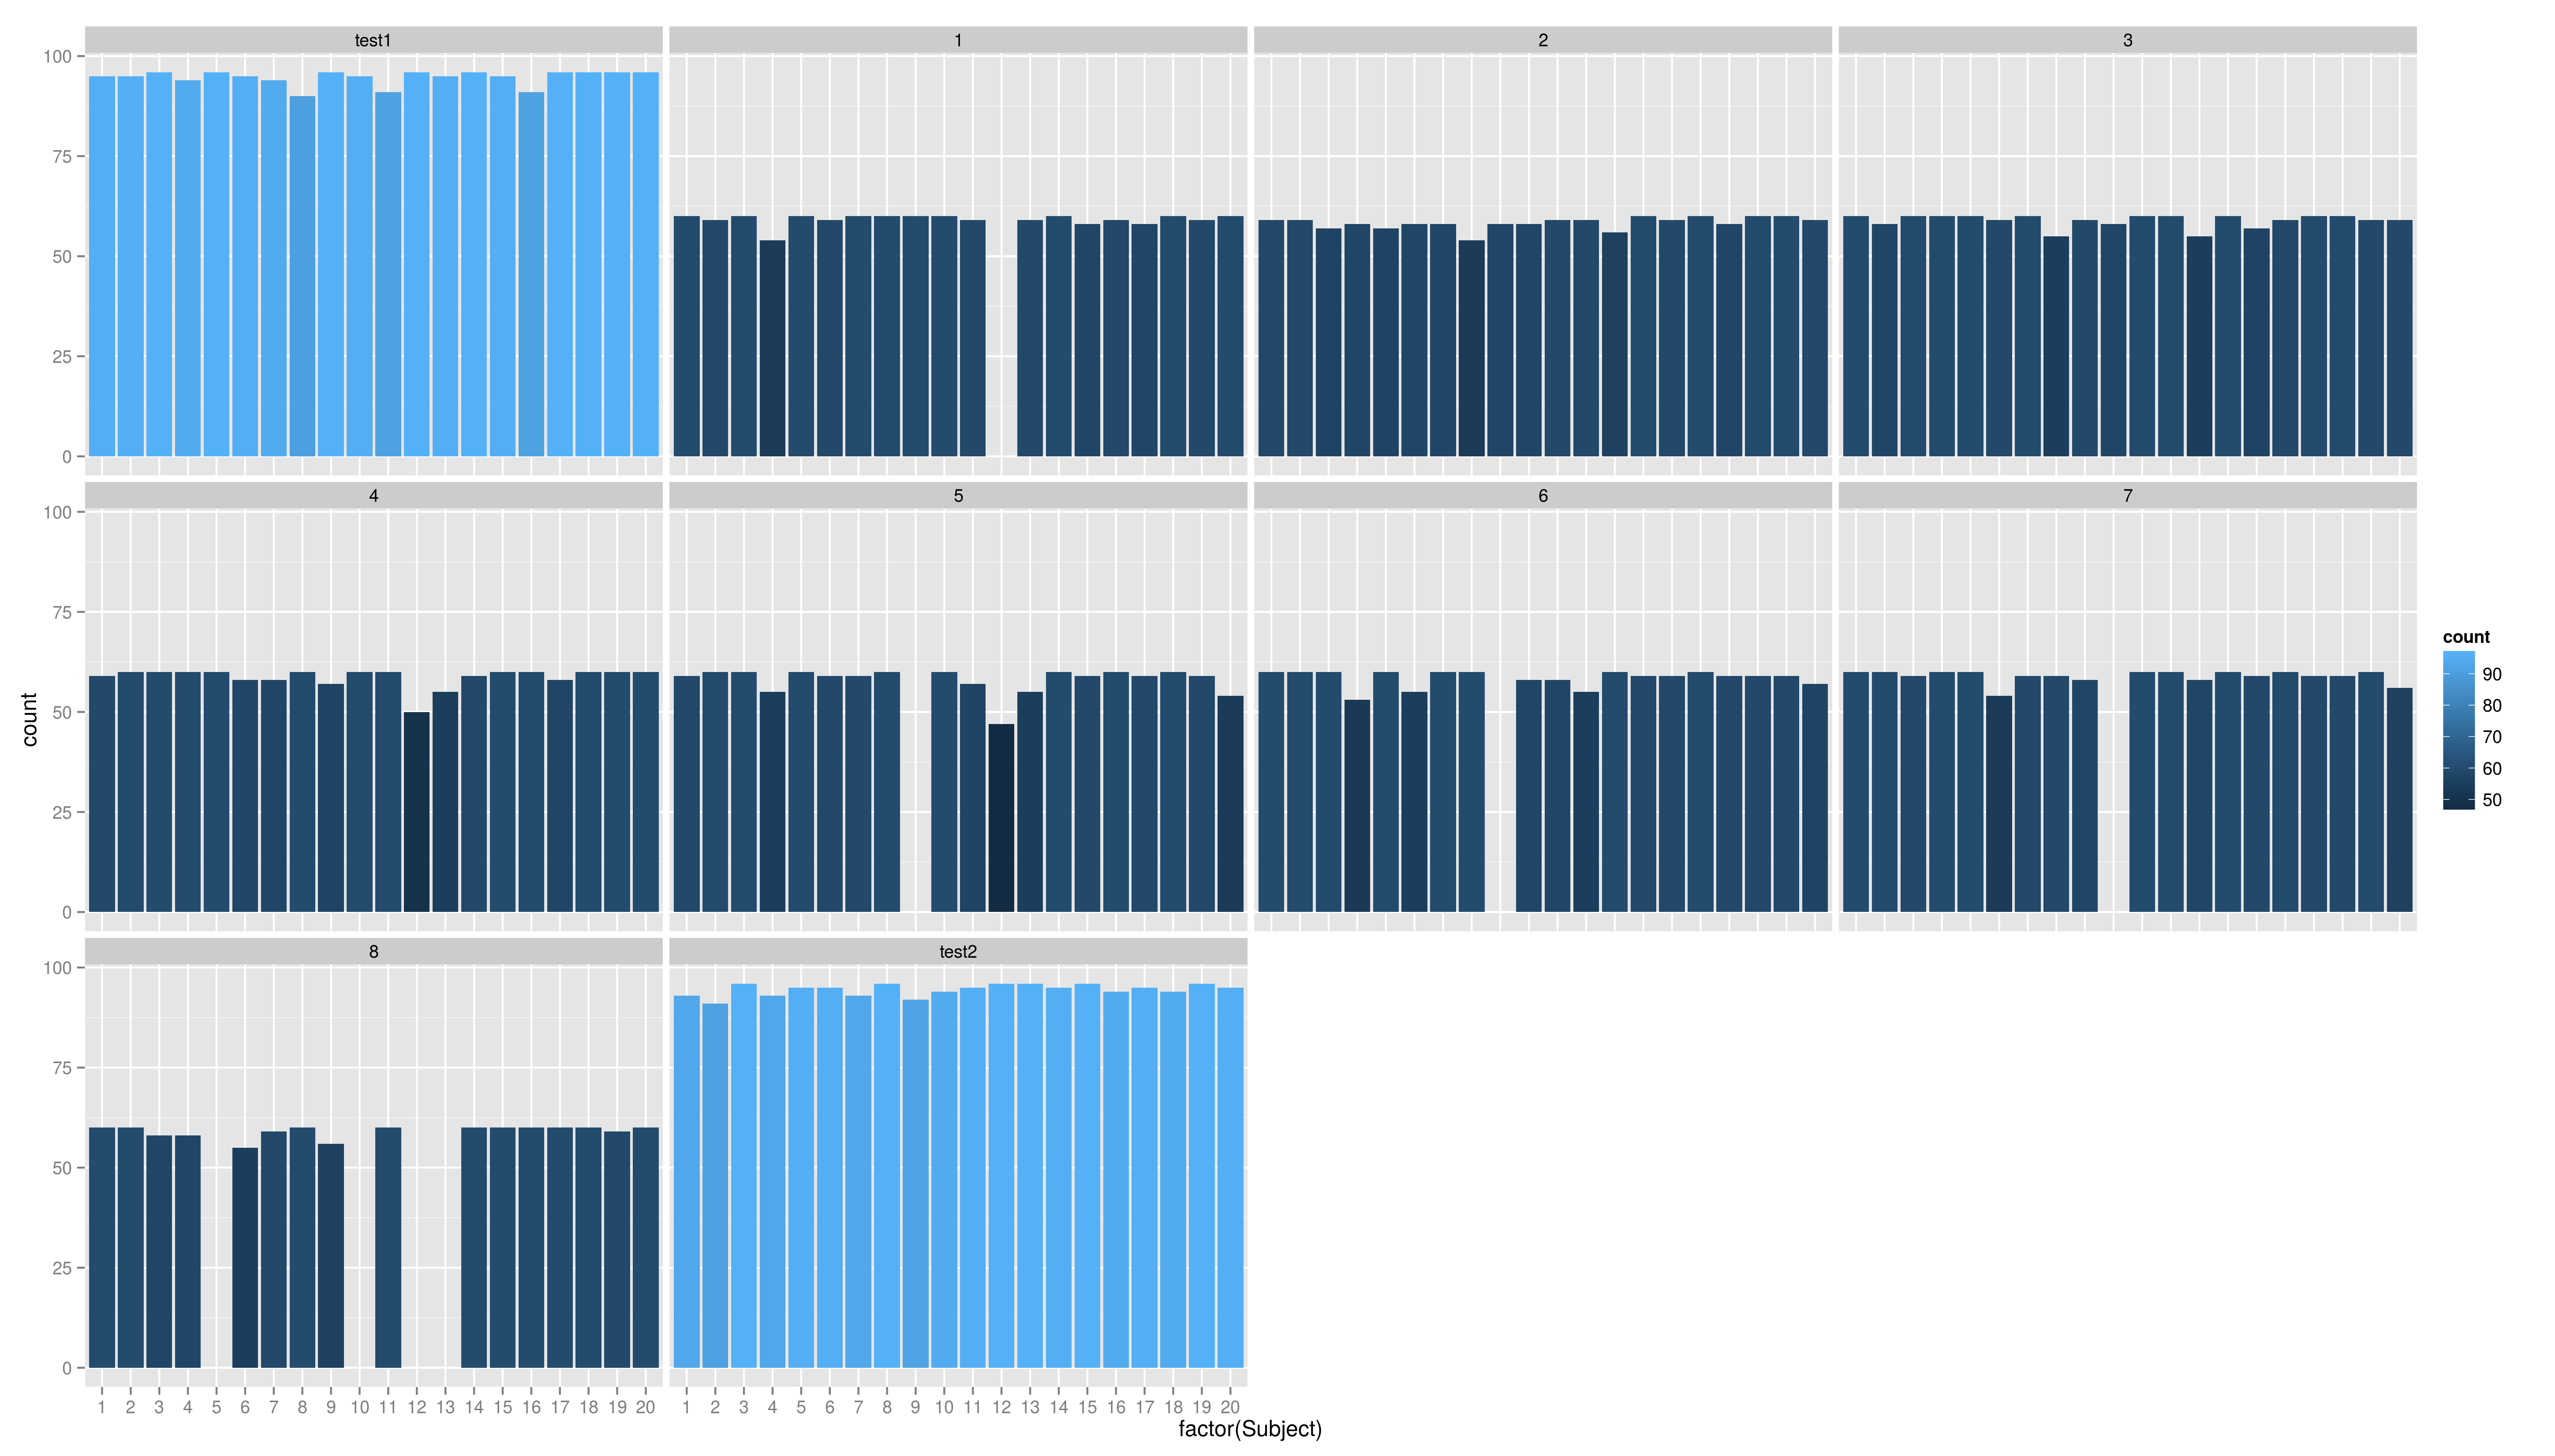
\includegraphics[width=8cm, height=4cm]{graph2.png}}{graph2.png}
\end{center}
\end{frame}

\begin{frame}[fragile]\frametitle{Summary Graphics}
And another one.
\begin{exampleblock}{Input/Output}\tiny
\begin{verbatim}
> ggplot(data,aes(x=testid,fill=Stim.Type)) +
+     geom_bar(position=position_fill()) +
+     facet_wrap(~Subject)
\end{verbatim}
    \end{exampleblock}
\begin{center}
  \linkimage{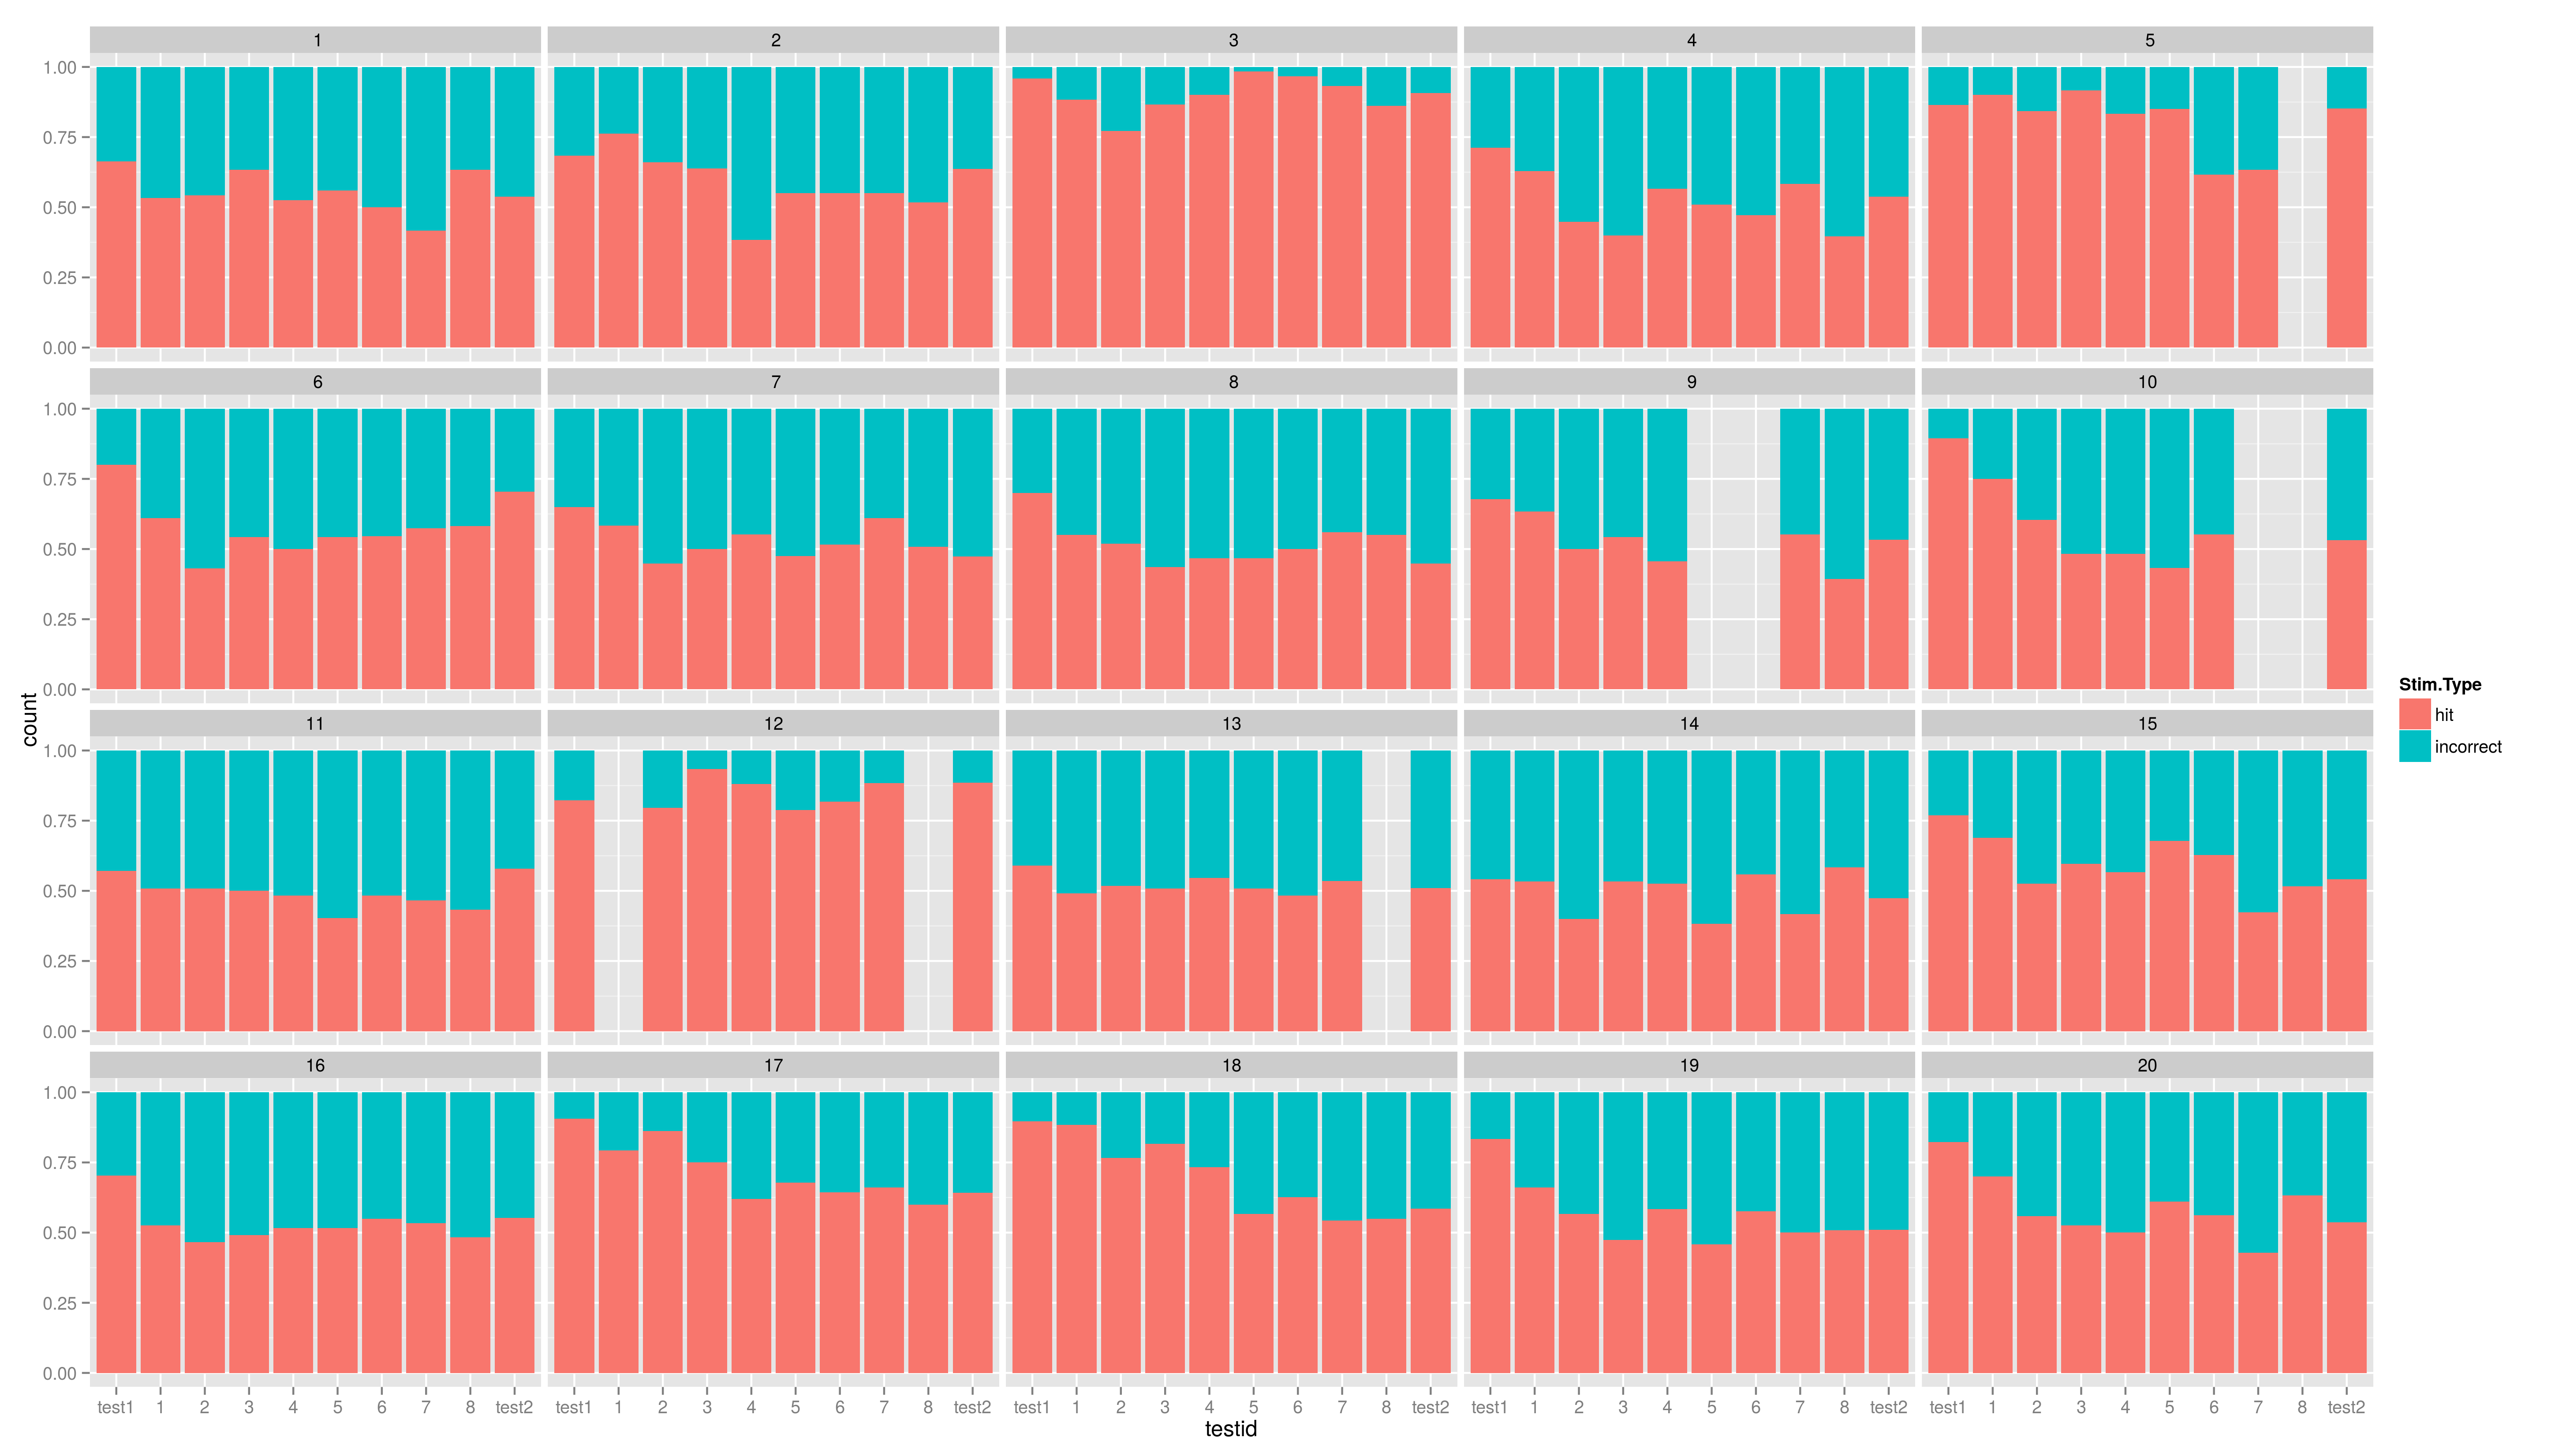
\includegraphics[width=8cm, height=4cm]{graph3.png}}{graph3.png}
\end{center}
\end{frame}


\appendix
\flushlinkimages

\end{document}
